\newpage
\section{Problem 5.7}
\subsection{重要参数}
\[f(x)=9x-4\ln(x-7)\]
\[g(x)=f'(x)=9-\dfrac{4}{x-7}\]
\[G(x)=g'(x)=\dfrac{4}{(x-7)^2}\]

其迭代公式为:
\begin{equation}
x^{(k+1)}=x^{(k)}-\dfrac{1}{4}(x^{(k)}-7)(9x^{(k)}-67)
\label{eq1}
\end{equation}


\subsection{算法伪代码}
\begin{algorithm}[h]  
\caption{Newton method for problem(5.7)}  
\begin{algorithmic}[1]  
\STATE Given $x^{(0)}$ and compute $g(x)=f'(x)$
\STATE Compute $G(x)=g'(x)$
\STATE Set $g^{(0)}=g(x^{(0)}),k=0$
\WHILE {$|g^{(k)}|>\epsilon$}
\STATE Set $s^{(k)}=-g^{(k)}/G^{(k)}$
\STATE Set $x^{(k+1)}=x^{(k)}+s^{(k)}$
\STATE Set k=k+1
\ENDWHILE
\end{algorithmic}  
\end{algorithm}  



\subsection{计算结果展示}
% Table generated by Excel2LaTeX from sheet 'Sheet1'
\begin{table}[htbp]
  \centering
  \caption{迭代5次过程}
    \begin{tabular}{clllll}
\toprule
  $x^{(0)}$&7.4  & 7.2  & 7.01 &7.80  & 7.88 \\
	\midrule
   $x^{(1)}$& 7.44  & 7.31  & 7.019775 & 7.16  & 7.0176 \\
    $x^{(2)}$&7.4444 & 7.403775 & 7.038670136 & 7.2624 & 7.03450304 \\
    $x^{(3)}$&7.44444444 & 7.440722936 & 7.073975668 & 7.36987904 & 7.066327546 \\
   $ x^{(4)}$&7.444444444 & 7.444413283 & 7.135638438 & 7.431934445 & 7.122756569 \\
    $x^{(5)}$&7.444444444 & 7.444444442 & 7.229881858 & 7.444092319 & 7.211607493 \\
	\midrule
    $f(x^{(5)})$&70.24372086 & 70.24372086 & 70.94969577 & 70.24372212 & 71.11655611 \\
	\bottomrule
    \end{tabular}%
  \label{tab:addlabel}%
\end{table}%

% Table generated by Excel2LaTeX from sheet 'Sheet1'
\begin{table}[htbp]
  \centering
  \caption{大范围迭代结果}
    \begin{tabular}{|c|c|c|c|}
    \hline
    初始点   & 迭代终止点 & 初始点   & 迭代终止点 \\
    \hline
    5     & -Inf  & 9     & -Inf \\
    \hline
    5.25  & -Inf  & 9.25  & -Inf \\
    \hline
    5.5   & -Inf  & 9.5   & -Inf \\
    \hline
    5.75  & -Inf  & 9.75  & -Inf \\
    \hline
    6     & -Inf  & 10    & -Inf \\
    \hline
    6.25  & -Inf  & 10.25 & -Inf \\
    \hline
    6.5   & -Inf  & 10.5  & -Inf \\
    \hline
    6.75  & -Inf  & 10.75 & -Inf \\
    \hline
    7     & 7     & 11    & -Inf \\
    \hline
    7.25  & 7.44444444444445 & 11.25 & -Inf \\
    \hline
    7.5   & 7.44444444444445 & 11.5  & -Inf \\
    \hline
    7.75  & 7.44444444444445 & 11.75 & -Inf \\
    \hline
    8     & -Inf  & 12    & -Inf \\
    \hline
    8.25  & -Inf  & 12.25 & -Inf \\
    \hline
    8.5   & -Inf  & 12.5  & -Inf \\
    \hline
    8.75  & -Inf  & 12.75 & -Inf \\
    \hline
    \end{tabular}%
  \label{tab:addlabel}%
\end{table}%


由MATLAB函数fminsearch求得最优解为:\[x^{\star}=7.444421386718750,\quad f(x^{\star})=70.243720870248540\]


\subsection{收敛域内点的迭代情况}
\begin{figure}[H]
\centering
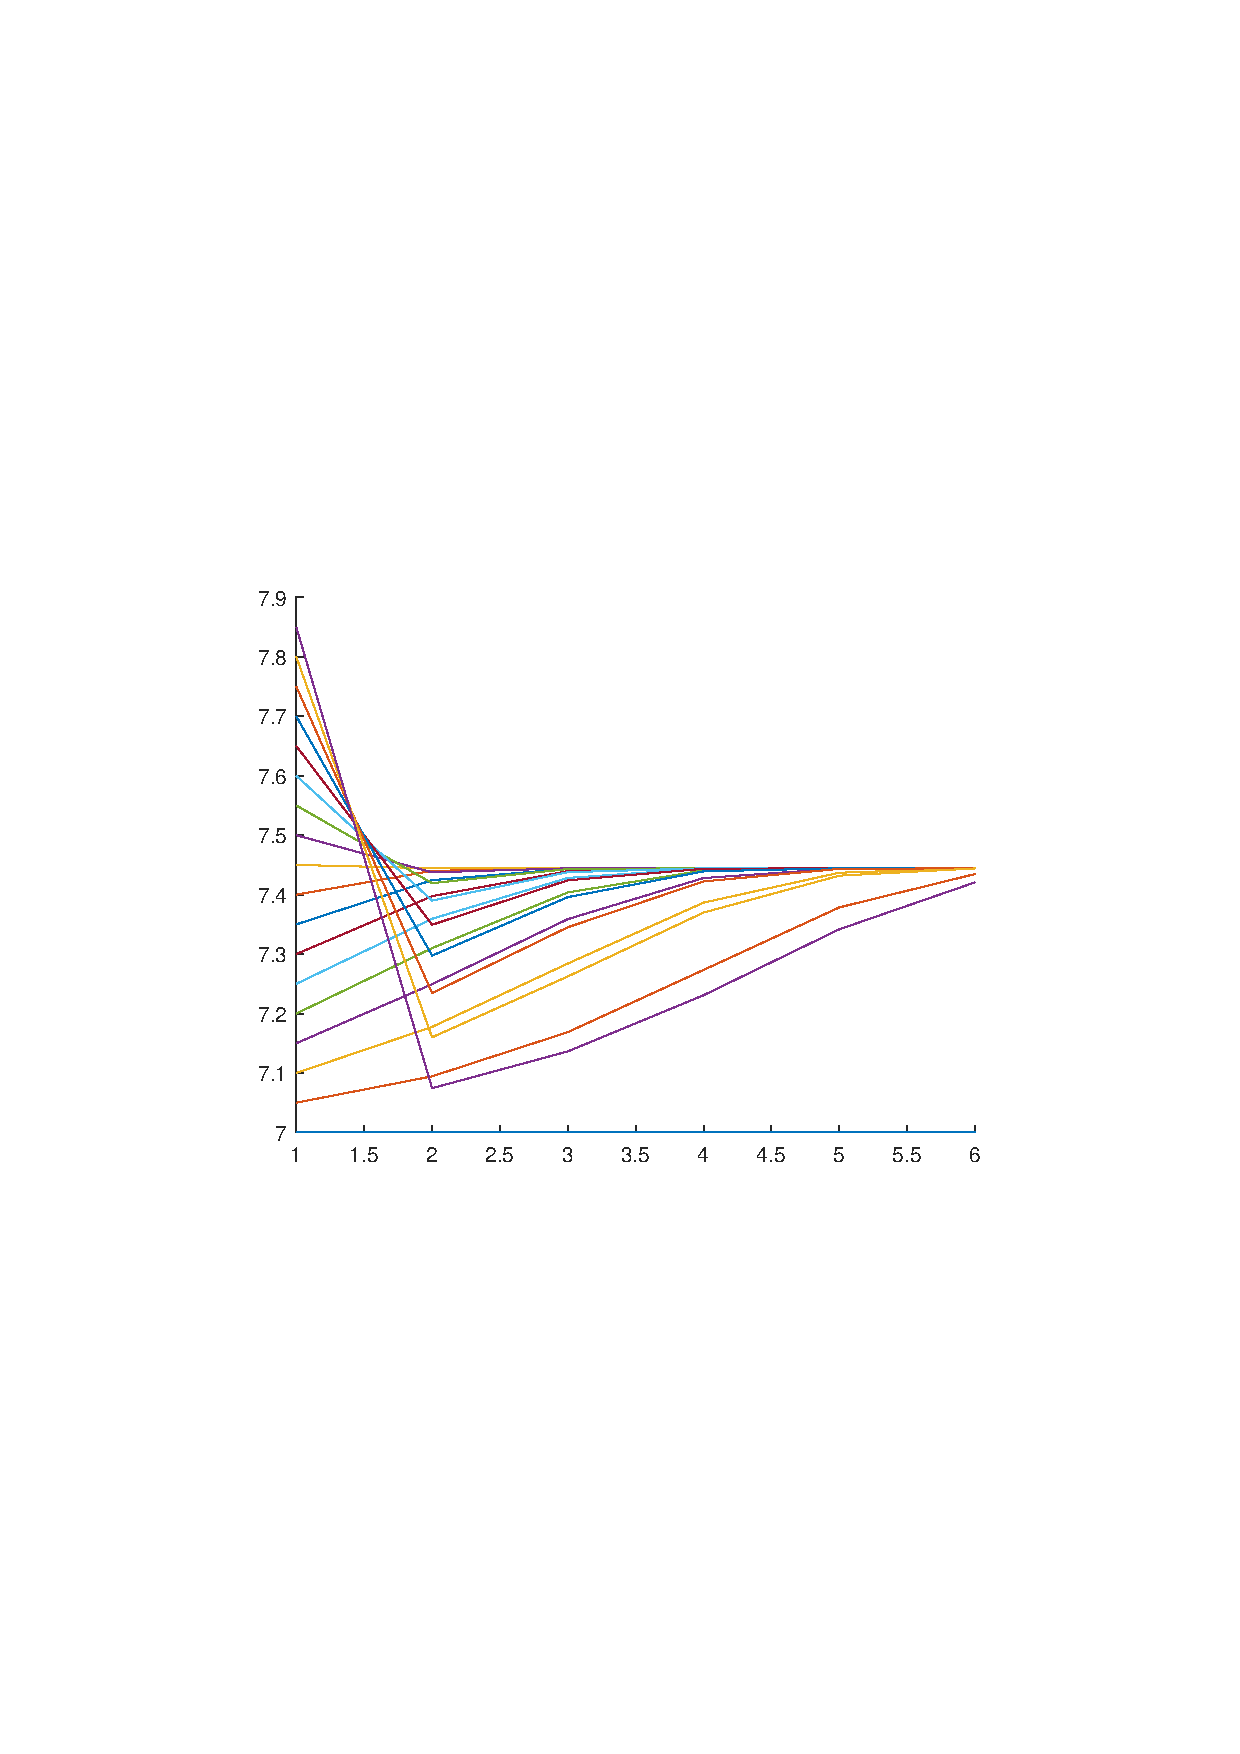
\includegraphics[width=10cm]{fig/2_1.pdf}
\end{figure}

\begin{figure}[H]
\centering
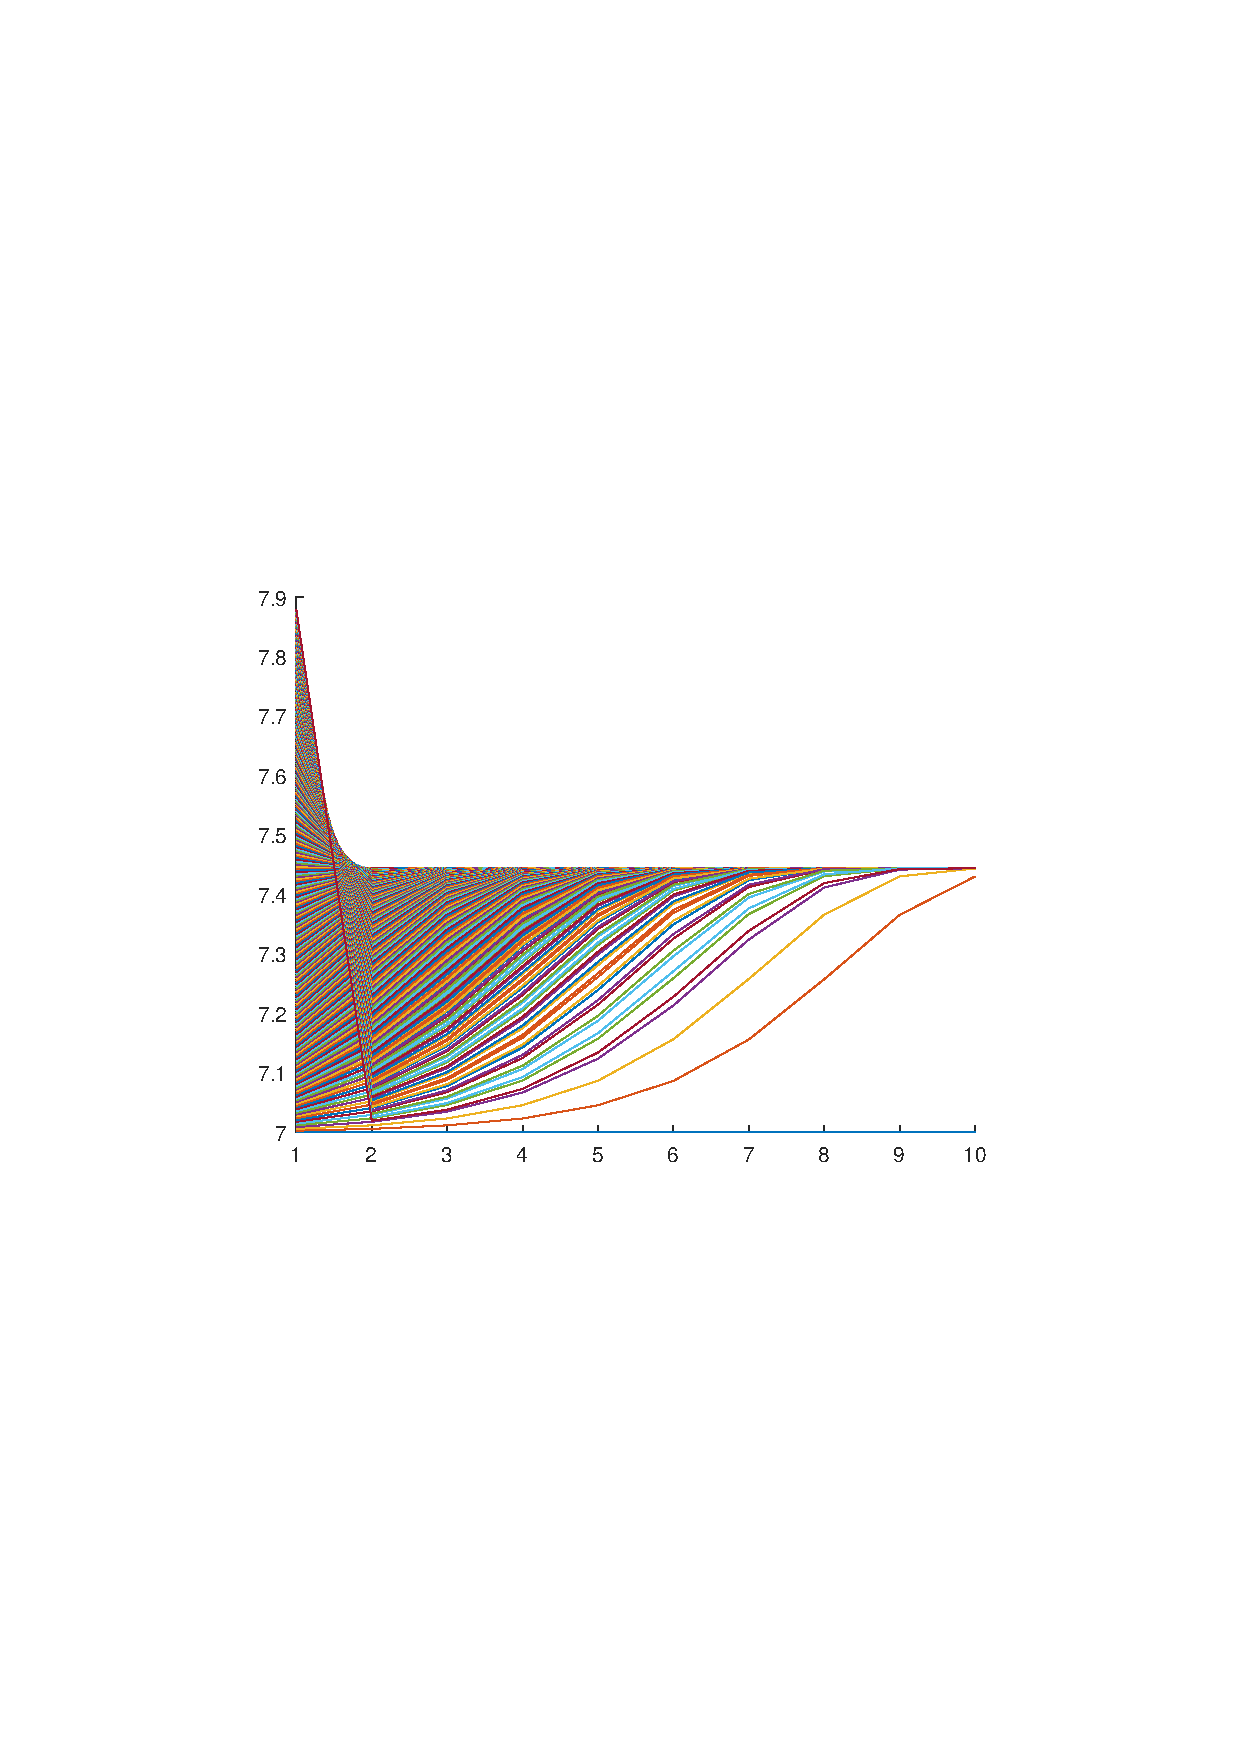
\includegraphics[width=10cm]{fig/2_2.pdf}
\end{figure}

\begin{figure}[H]
\centering
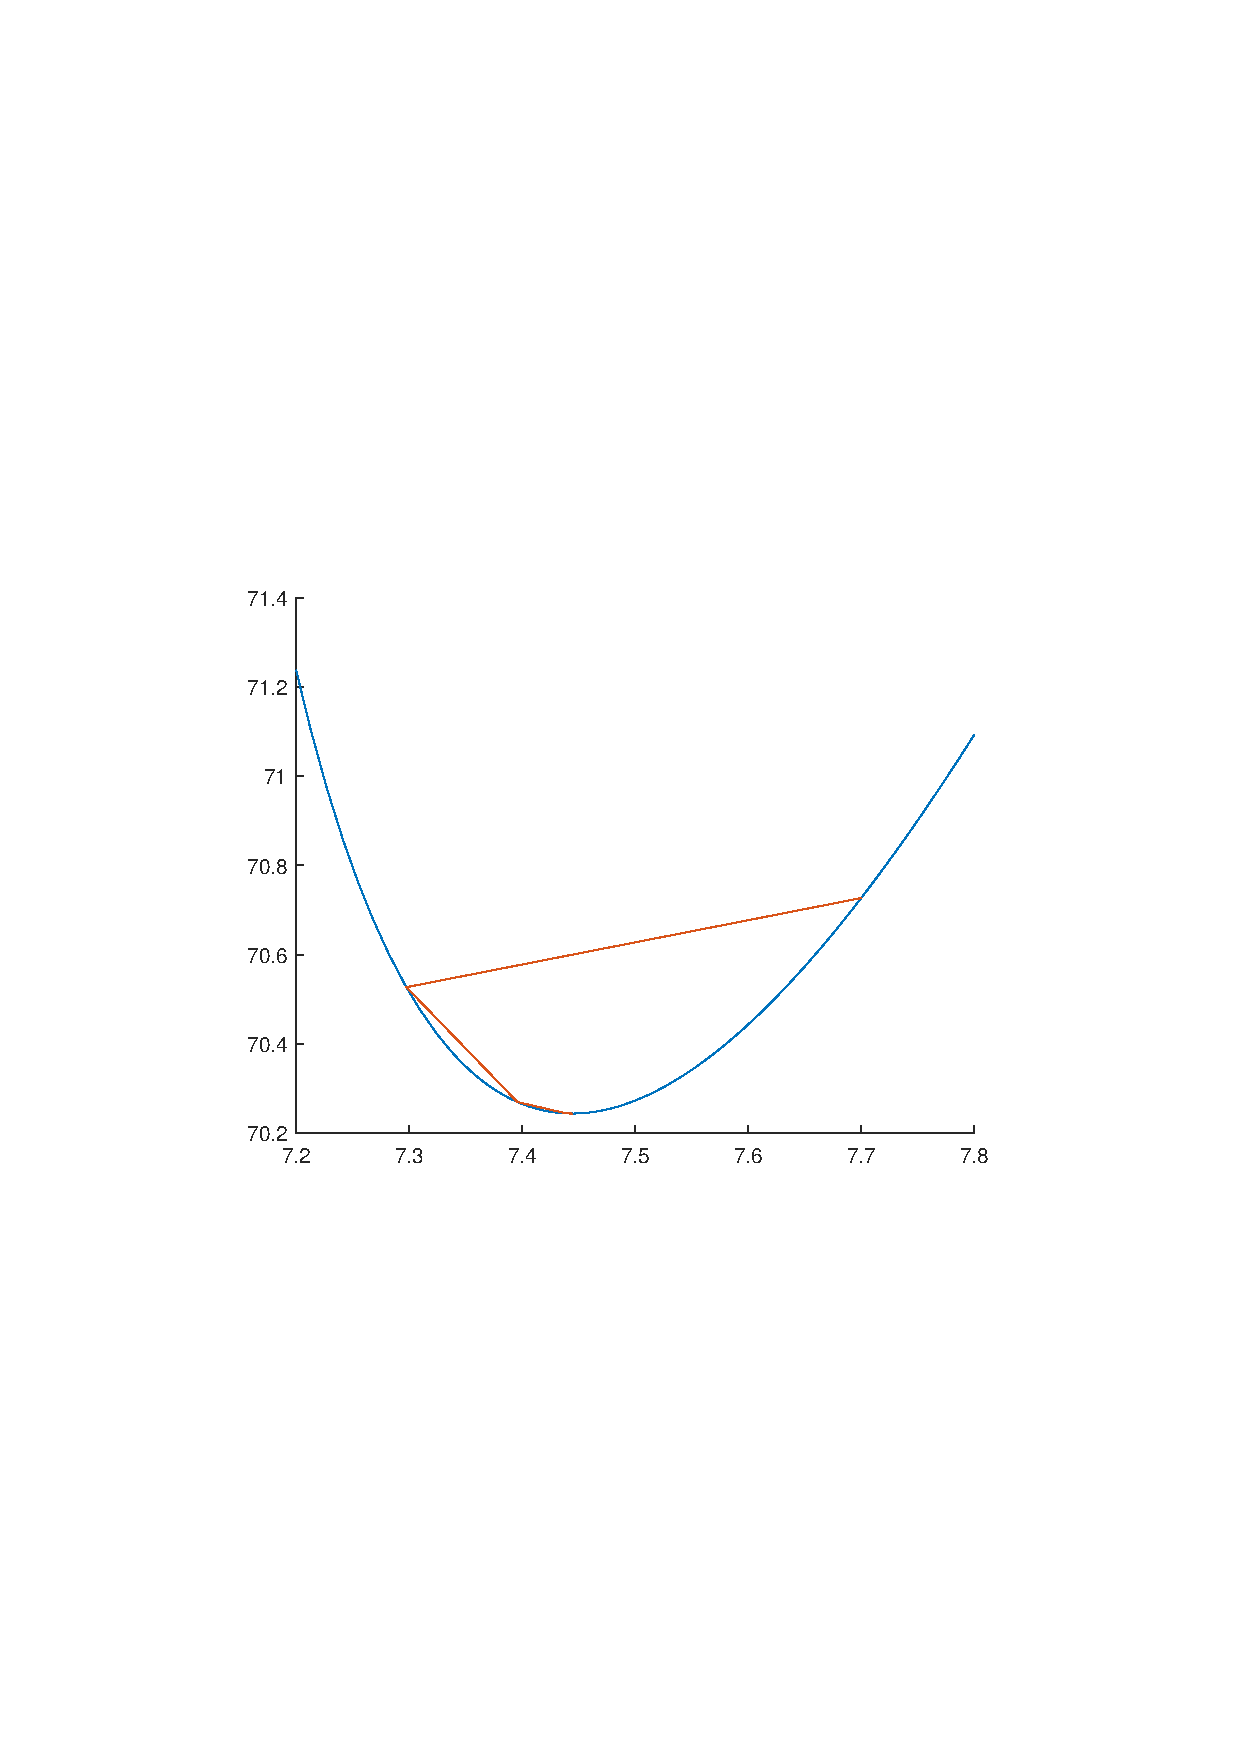
\includegraphics[width=11cm]{fig/2_3.pdf}
\end{figure}

%\newpage
\subsection{总结分析}
\subsection*{关于收敛域的分析}

首先由于$G(x)>0$,故在定义域内总能收敛。

然后我们观察迭代公式(equation:\ref{eq1})
\[x^{(k+1)}=x^{(k)}-\dfrac{1}{4}(x^{(k)}-7)(9x^{(k)}-67)\]
可以得出以下结论:
\begin{itemize}
\item
容易看出两个稳定点为$x'=7\ and\ x^{\star}=67/9$
\item
若初始点在定义域内,则要求$x_0>=7$
\item
然后要避免$x_k$迭代时使得$x^{(k+1)}$跳出定义域,
因此解方程
\[7=x^{(k)}-\dfrac{1}{4}(x^{(k)}-7)(9x^{(k)}-67)\]

得到解:$x_k=7\ or \ 71/9$
\item
因此该迭代公式的收敛域为$(7,71/9)$
\end{itemize}

\subsection*{点的迭代性质分析}
观察点的迭代图像可以看到:
\begin{itemize}
\item
在收敛域$(7,71/9)$内$x$将逐渐收敛到稳定点$x^{\star}=67/9$
\item
若起始点$x_0\in (67/9,71/9)$,则其迭代第一步的步长非常大,使得一下子就跃到$67/9$以下,然后慢慢朝稳定点方向靠近,而且一开始离稳定点越大,步长越大,这可由公式(equation:\ref{eq1})解释

\item
但当$x_0$离稳定点太远,超出$71/9$时,将会使得下一步迭代步长过大,导致超出定义域。

\item
若起始点$x_0\in (7,67/9)$时,$x_0$不会像之前那样猛烈地向稳定点$x^{\star}$迈进,而是缓慢地迭代,而越远离稳定点$x^{\star}$,迭代得越慢

\item
透过公式(equation:\ref{eq1}),我们可以用一种形象的语言来描述这种现象:当$x_0>67/9$时,它受到了两个稳定点$x',x^{\star}$的“吸引”,因此迈出的步长特别大。而当$7<x_0<67/9$时,$x^{\star}$对它的“吸引力”被另一个稳定点$x'$的“吸引力”抵消了一部分,而离$x'$越近,“引力”被抵消得越厉害,迭代也就越慢.
\end{itemize}







